%% osm-technique.tex



\frame[plain]{  \heading{Plan de la Présentation}
\ecmsetupplan
\begin{itemize}
  \item[\small $\Diamond$] Introduction
  \item[\small $\Diamond$] Fonctionnement 
  \item[\small $\Diamond$] Applications
  \item[\small $\Diamond$] {\color{purple}\textbf{Technique}}
  \item[\small $\Diamond$] Communauté
  \item[\small $\Diamond$] Conclusions
\end{itemize}
}


\tikzstyle{data} = [draw,rounded corners,fill=blue!20]
\tikzstyle{database} = [draw,cylinder,shape border rotate=90,aspect=0.07,fill=purple!40]
\tikzstyle{tool} = [draw,thin,fill=green!30,text centered,drop shadow]




\frame { \heading{Composants logiciels} \vfill

\begin{tikzpicture}[auto,>=latex',font={\sffamily\tiny}]
    \node[data] (0,0) (GPS) {traces GPS};
    \node[data,right of=GPS,node distance=1.5cm] (yahoo) {imagerie Yahoo!};
    \node[data,right of=yahoo,node distance=1.5cm] (cadastre) {cadastre};
    \node[coordinate,below of=yahoo,node distance=0.5cm] (data) {};
    \node[tool,below of=data,xshift=-0.6cm,node distance=0.5cm] (JOSM) {JOSM};
    \node[tool,below of=data,xshift=0.6cm,node distance=0.5cm] (potlatch) {Potlatch};
    \path[draw] (GPS) -- (data);
    \path[draw] (yahoo) --  (data);
    \path[draw] (cadastre) -- (data);  
    \path[draw,->] (data) -- (JOSM);
    \path[draw,->] (data) -- (potlatch);
    \pause
    
    \node[tool,below of=data,node distance=1.5cm] (API) {API 0.6};
    \path[draw,<->] (JOSM) -- node[yshift=-0.2cm] {REST} (API);
    \path[draw,<->] (potlatch) -- (API);

    \node[database,below of=API] (PG) {backend PostgreSQL};
    \path[draw,<->] (API) -- (PG);
    \pause

    \node[data,left of=API,node distance=1.5cm] (geodata) {données GIS};
    \path[draw,->] (geodata) -- (API);
    \pause
    
    \node[tool,right of=PG,node distance=2cm] (osmosis) {osmosis};
    \path[draw,->] (PG) -- (osmosis);
    \node[database,right of=osmosis,node distance=2cm] (planet) {dumps ``planet''};
    \path[draw,->] (osmosis) -- (planet);
    \pause
    
    \node[tool,above of=planet] (osm2pgsql) {osm2pgsql};
    \path[draw,->] (planet) -- (osm2pgsql);
    \node[database,above of=osm2pgsql] (postgis) {PostGIS};
    \node[right of=postgis] {
\includegraphics[height=0.8cm]{figures/postgis-logo}};
    \path[draw,->] (osm2pgsql) -- (postgis);
    \node[above of=postgis] (mapnik)
    {
\includegraphics[width=1.6cm]{figures/mapnik-logo}};
    \path[draw,->] (postgis) -- (mapnik);
    \node[tool,right of=mapnik,node distance=1.8cm] (style) {feuilles de style};
    \path[draw,->] (style) -- (mapnik);
    \node[database,above of=mapnik,node distance=1cm,text width=1.1cm,text centered]
      (tiles) {tuiles (mod\_tile)};
    \path[draw,->] (mapnik) -- (tiles);
    \node[above of=tiles,node distance=1.1cm] (slippy)
    {
\includegraphics[width=0.7cm]{figures/OpenLayers-logo}\hskip-0.8cm\raisebox{17pt}{OpenLayers}};
    \path[draw,->] (tiles) -- (slippy);
    \node[right of=slippy,node distance=2cm] (browser){
\includegraphics[width=0.7cm]{figures/firefox-logo}};
    \path[draw,<-] (slippy) -- (browser);
    \pause
    
    \node[tool,right of=planet,node distance=2cm] (XAPI) {XAPI};
    \path[draw,->] (planet) -- (XAPI);
    \node[tool,right of=planet,node distance=2cm,yshift=1cm] (namefinder) {namefinder};
    \path[draw,->] (planet) -- (namefinder);
    \node[database,below of=planet,node distance=0.7cm] (mirror) {planet mirrors};
    \path[draw,->] (planet) -- (mirror);
\end{tikzpicture}
}


%% http://svn.openstreetmap.org/applications/utils/osmosis/trunk/script/contrib/apidb_0.6.sql
%% http://wiki.openstreetmap.org/wiki/Database_schema
%% http://en.wikipedia.org/wiki/Morton_number_(number_theory)
\frame { \heading{Backend PostgreSQL} \vfill

  Contient les données actuelles et historiques, les fichiers GPX
  
  \begin{itemize}
  \item 1.23 To sur disque (dont 690 Go pour l'historique, 100 Go pour les
  points GPS)
  
  \item Moyenne de 3 millions de tuples lus par seconde

  \item Moyenne de 500 ajouts/modifs/suppressions par seconde

  \item Utilisation de quadtiles pour accélérer les recherches  % FIXME expand

  \item Système de diffs (par minute, heure, jour) pour permettre à
  d'autres de se synchroniser
  \end{itemize}
}

\begin{frame}[fragile]{Format XML planet}
\tiny
\begin{verbatim}
<?xml version='1.0' encoding='UTF-8'?>
<osm version="0.5" generator="Osmosis 0.26">
  <bound box="41.33878,-5.14222,51.09280,9.56156" origin="http://www.openstreetmap.org/api/0.5"/>
 <node id="475037" timestamp="2008-09-18T07:33:10Z" user="HeikoE" lat="48.4949265" lon="7.7839893"/>
  <node id="475038" timestamp="2008-09-18T07:33:10Z" user="HeikoE" lat="48.4946876" lon="7.7814487"/>
  <node id="477010" timestamp="2008-09-18T07:33:10Z" user="Pieren" lat="48.4607686" lon="7.5112136"/>
  <node id="477015" timestamp="2008-09-18T07:33:10Z" user="Pieren" lat="48.4671357" lon="7.5124533"/>
  ...
 <way id="2788576" timestamp="2008-09-18T07:33:10Z" user="Alban">
    <nd ref="12606591"/>
    <nd ref="14471355"/>
    <nd ref="12606592"/>
    <tag k="name" v="Rue Antoine de Saint Exupery"/>
    <tag k="created_by" v="Editop"/>
    <tag k="highway" v="residential"/>
  </way>
  ...
   <relation id="960" timestamp="2008-09-18T07:33:10Z" user="Drexl">
    <member type="way" ref="8157759" role=""/>
    <member type="way" ref="8157772" role=""/>
    <tag k="type" v="multipolygon"/>
    <tag k="created_by" v="Potlatch 0.9c"/>
  </relation>
\end{verbatim}
\end{frame}



\begin{frame}[fragile]{Fonctionnement API} \vfill

Racine des requêtes: \url{http://api.openstreetmap.org/} \bigskip

\texttt{GET /api/0.6/map?bbox={\color{purple}left},{\color{purple}bottom},{\color{purple}right},{\color{purple}top}}

{\tiny
\begin{verbatim}
<?xml version='1.0' encoding='UTF-8'?>
<osm version="0.6">
  <bound box="41.33878,-5.14222,51.09280,9.56156" origin="http://www.openstreetmap.org/api/0.5"/>
 <node id="475037" timestamp="2008-09-18T07:33:10Z" user="HeikoE" lat="48.4949265" lon="7.7839893"/>
  <node id="475038" timestamp="2008-09-18T07:33:10Z" user="HeikoE" lat="48.4946876" lon="7.7814487"/>
  <node id="477010" timestamp="2008-09-18T07:33:10Z" user="Pieren" lat="48.4607686" lon="7.5112136"/>
</osm>
\end{verbatim}
}
\bigskip

\texttt{GET /api/0.6/[{\color{purple}node|way|relation}]/\#id}

{\tiny
\begin{verbatim}
<node id="123" lat="..." lon="..." version="142" changeset="12" user="fred" uid="123" timestamp="...">
  <tag k="note" v="Just a node"/>
  ...
</node>
\end{verbatim}
}

\end{frame}


\begin{frame}[fragile]{Fonctionnement API} \vfill

\texttt{PUT /api/0.6/changeset/create}
{\small
\begin{verbatim}
<osm>
  <changeset>
    <tag k="created_by" v="JOSM 1.61"/>
    <tag k="comment" v="Just adding some streetnames"/>
    ...
  </changeset>
  ...
</osm>
\end{verbatim}
}

\bigskip

\texttt{PUT /api/0.6/[{\color{purple}node|way|relation}]/create}
{\small
\begin{verbatim}
<node changeset="12" lat="..." lon="...">
  <tag k="note" v="Just a node"/>
  ...
</node>
\end{verbatim}
}
\end{frame}


\tikzstyle{what}    = [baseline,rounded corners,outer sep=3pt,inner sep=2pt,fill=blue!20]
\tikzstyle{explain} = [text width=3cm,anchor=base,fill=red!20,text centered,font={\sffamily\tiny}]
\tikzstyle{epath}   = [->,thin,dotted]


\frame{\heading{osm2pgsql} \vfill\small

Prend un dump planet (ou extrait) et le charge dans une base PostGIS,
selon critères de filtrage
\begin{itemize}
\item processus très gourmand en RAM!
\end{itemize}

Au final, la base contient des tables:

\begin{itemize}
\item \texttt{planet\_osm\_line}: chemins de fer, métro, ...
\item \texttt{planet\_osm\_point}: stations de métro, magasins, banques, ...
\item \texttt{planet\_osm\_polygon}: parks, lacs, bâtiments, ...
\item \texttt{planet\_osm\_roads}: uniquement les routes
\end{itemize}

Mapnik intérroge la base PostGIS pour générer les cartes
\begin{itemize}
\item à la volée avec \texttt{mod\_tile} 
\item en pré-rendu
\end{itemize}

Feuilles de style mapnik permettent de personnaliser le rendu (si
compatible avec filtrage osm2pgsql)
}


\begin{frame}[fragile]{Requêtes GIS avec PostGIS} \vfill

Où aller se rafraîchir après l'apéritif de clôture?

\begin{verbatim}
SELECT
  p.name,
  ST_Distance(ST_Transform(p.way,3348),
  ST_Transform(u.way,3348) )
  FROM planet_osm_point p, planet_osm_point u
  WHERE p.amenity = 'pub'
  AND u.name='ENSEEIHT' AND
  ST_Distance(p.way,u.way) < 1;
\end{verbatim}

\end{frame}


\begin{frame}[fragile]{Données OSM dans OpenJUMP} \vfill
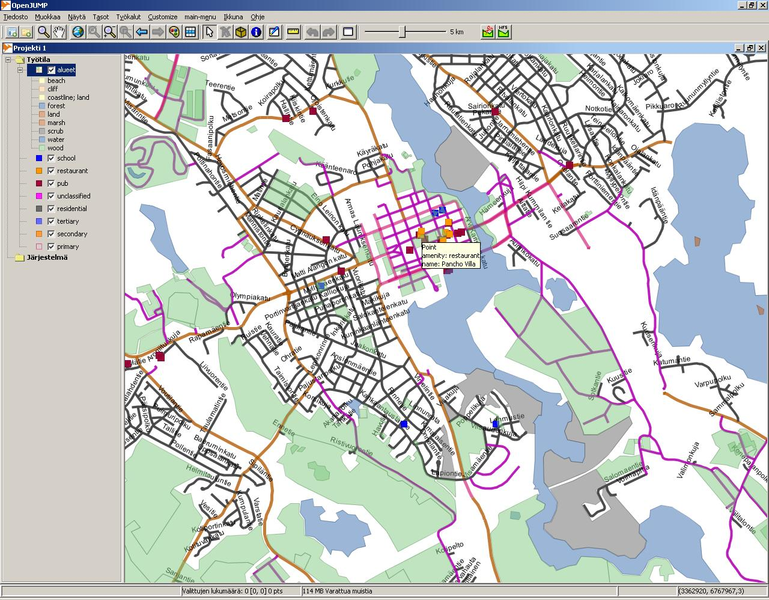
\includegraphics[width=0.8\textwidth]{figures/osm-openjump}
\end{frame}


%% EOF
